\begin{question}
Given the historical series of three stock prices in the file
\(\href{https://raw.githubusercontent.com/matteosan1/finance_course/develop/libro/input_files/historical.csv}{\textrm{historical.csv}}\)
compute the 1-day 95\% VaR for a portfolio consisting of 40 FOX shares, 35 ABC shares and 25 CBS shares. 
Today's price is the last entry of the series.

\noindent\textbf{Hint:} when simulating the historical scenarios take care of possible NaN values
in the series. 
\end{question}

\cprotEnv\begin{solution}
\begin{ipython}
import pandas as pd
from scipy.stats import norm

df = pd.read_csv("historical.csv")
fox = df[df['ticker']=='FOX'].copy()
cbs = df[df['ticker']=='CBS'].copy()
abc = df[df['ticker']=='ABC'].copy()
fox['rets'] = fox['adj_close']/fox['adj_close'].shift(1) - 1
cbs['rets'] = cbs['adj_close']/cbs['adj_close'].shift(1) - 1
abc['rets'] = abc['adj_close']/abc['adj_close'].shift(1) - 1

print (fox.head())
\end{ipython}
\begin{ioutput}
None      date ticker adj_close      rets
0 0 2018-03-27    FOX     36.08       NaN
1 1 2018-03-26    FOX     36.58  0.013858
2 2 2018-03-23    FOX     35.45 -0.030891
3 3 2018-03-22    FOX     36.18  0.020592
4 4 2018-03-21    FOX     36.30  0.003317
\end{ioutput}
\begin{ipython}
w = np.array([0.4, 0.35, 0.25])
rets = []
for i in range(1, len(abc)):
    ret = [fox.iloc[i]['rets'], abc.iloc[i]['rets'],
           cbs.iloc[i]['rets']]
    if np.NaN in ret:
        continue
    rets.append(w[0]*ret[0] + w[1]*ret[1] + w[2] * ret[2])

current_price = [fox.iloc[-1]['adj_close'],
                 abc.iloc[-1]['adj_close'],
                 cbs.iloc[-1]['adj_close']]
portfolio_price = w.dot(current_price)
hist_var = portfolio_price*np.percentile(rets, 1)
print ('Historical VAR is {:.3f}'.format(hist_var))
\end{ipython}
\begin{ioutput}
Historical VAR is -1.385
\end{ioutput}
\begin{figure}[htbp]
	\centering
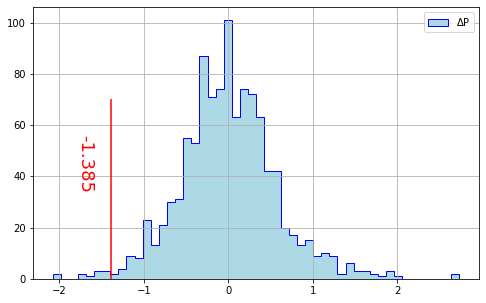
\includegraphics[width=0.7\linewidth]{figures/hist_var_ex}
\end{figure}
\end{solution}

\begin{question}
You have a 3-years call with strike \euro{110}. The underlying initial price is \euro{100} and the mean rate of return is 0.05 with a volatility of 0.15. The risk-free rate is 0.03 flat.
Compute the CVA of the contract assuming a recovery rate of 40\% and default probabilities for the underlying of 10\%, 20\% and 30\% for first, second and third year respectively.
\end{question}

\cprotEnv\begin{solution}
Below ten simulations of the underlying price in the next three years.

\begin{figure}[htbp]
	\centering
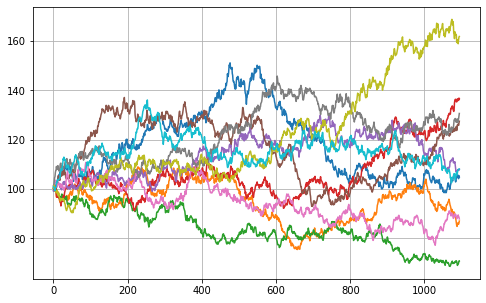
\includegraphics[width=0.7\linewidth]{figures/underlying_simulation}
\end{figure}
This is a first implementation of the CVA calculation, not optimized in terms of speed. It takes about 700 seconds to run 1000 simulations.

\begin{ipython}
from datetime import date
from dateutil.relativedelta import relativedelta
from finmarkets import call_price, CreditCurve
from scipy.stats import norm
import numpy as np
import time

np.random.seed(1)
dt = 1/365
K = 110
sigma = 0.15
mu = 0.05
r = 0.03
T = 3
R = 0.4
S = [1, 0.9, 0.8, 0.7]
obs_date = date.today()
pillars = [obs_date + relativedelta(years=i) for i in range(T+1)]
cc = CreditCurve(pillars, S)
t1 = time.time()
scenarios = 1000
cvas = []
St = S0*np.ones(shape=(T*365, scenarios))
for s in range(scenarios):
    cva = 0
    St = 100
    for t in range(0, 365*T):
        St = St * np.exp((mu - 0.5 * sigma**2) * dt + sigma
            * np.sqrt(dt) * norm.rvs(size=1))
        cva += call_price(dt*t, St, K, r, sigma, T)
            *(cc.ndp(obs_date+relativedelta(days=t))-
            cc.ndp(obs_date+relativedelta(days=t+1)))

        cvas.append(cva*(1-R))

print (np.mean(cvas))
print (time.time()-t1)
\end{ipython}
\begin{ioutput}
\end{ioutput}
The next implementation, the one actually used, exploits the \texttt{numpy.array} and it is about 30\% faster.

\begin{ipython}
from datetime import date
from dateutil.relativedelta import relativedelta
from finmarkets import call_price, CreditCurve
from scipy.stats import norm
import numpy as np
import time

np.random.seed(1)
dt = 1/365
K = 110
sigma = 0.15
mu = 0.05
r = 0.03
T = 3
R = 0.4
S = [1, 0.9, 0.8, 0.7]
obs_date = date.today()
pillars = [obs_date + relativedelta(years=i) for i in range(T+1)]
cc = CreditCurve(pillars, S)
t1 = time.time()
scenarios = 1000
cvas = []
St = S0*np.ones(shape=(T*365, scenarios))
for i in range(T*365):
    norms = norm.rvs(size=scenarios)
    St[i, :] = St[i-1, :] * np.exp((mu - 0.5 * sigma**2) * dt + sigma
        * np.sqrt(dt) * norms[:])

for s in range(scenarios):
    cva = 0
    for t in range(365*T):
        cva += call_price(dt*t, St[i, s], K, r, sigma, T)* \
            (cc.ndp(obs_date+relativedelta(days=t))-
             cc.ndp(obs_date+relativedelta(days=t+1)))

        cvas.append(cva*(1-R))

print (np.mean(cvas))
print (time.time()-t1)
\end{ipython}
\begin{ioutput}
3.7521017896018973
459.46695613861084
\end{ioutput}
\end{solution}

\begin{question}
Consider a 1-years call with strike \euro{110}. The underlying initial price is \euro{100} and the mean rate of return is 0.05 with a volatility of 0.15. The risk-free rate is 0.03 flat.
Compute the 99.9\% Credit VaR assuming a recovery rate of 40\% and default probabilities for the underlying of 30\% within next year.
\end{question}

\cprotEnv\begin{solution}

\begin{ipython}
# 460s for 1000 simulations
from datetime import date
from dateutil.relativedelta import relativedelta
from finmarkets import call_price, CreditCurve
from scipy.stats import norm
import numpy as np

np.random.seed(1)
dt = 1/365
K = 110
sigma = 0.15
mu = 0.05
r = 0.03
T = 1
R = 0.4
S = [1, 0.7]
obs_date = date.today()
pillars = [obs_date + relativedelta(years=i) for i in range(T+1)]
cc = CreditCurve(pillars, S)
scenarios = 1000
losses = []
St = S0*np.ones(shape=(T*365, scenarios))
for i in range(T*365):
    norms = norm.rvs(size=scenarios)
    St[i, :] = St[i-1, :] * np.exp((mu - 0.5 * sigma**2) * dt + sigma
        * np.sqrt(dt) * norms[:])

for s in range(scenarios):
    loss = 0
    for t in range(365*T):
        loss += call_price(dt*t, St[i, s], K, r, sigma, T)* \
            (cc.ndp(obs_date+relativedelta(days=t))-
             cc.ndp(obs_date+relativedelta(days=t+1)))

        losses.append(cva*(1-R))

print (np.percentile(cvas, [99.9]))
\end{ipython}
\begin{ioutput}
[9.96586061]
\end{ioutput}

\begin{figure}[htbp]
	\centering
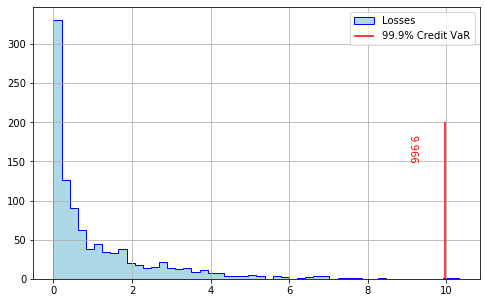
\includegraphics[width=0.7\linewidth]{figures/cr_var_ex}
\end{figure}
\end{solution}





